\subsection{Setup and Data Loading}

To initiate the analysis, it was essential to first examine the structure of the dataset. The dataset contains private messages exchanged on an online social network at UC Irvine. Each entry represents a message characterized by the following attributes:

\begin{itemize}
    \item \texttt{SRC}: Identifier of the sender
    \item \texttt{TGT}: Identifier of the receiver
    \item \texttt{UNIXTS}: Timestamp of the message in Unix time format
\end{itemize}

Given the non-human-readable format of UNIX timestamps, these were converted into datetime objects. To ensure temporal accuracy in the context of UC Irvine, all timestamps were further adjusted from UTC to the Pacific Time Zone (America/Los\_Angeles), accounting for daylight saving time.

\subsection{Data Exploration}

As an initial step, the following questions were posed: \textit{"How large is the dataset? How many users are involved and over what time span does the activity occur?"}

\begin{itemize}
    \item Total number of messages: 59,835
    \item Total number of unique users: 1,899
    \item Temporal coverage: From April 15, 2004 to October 26, 2004
\end{itemize}

These findings confirmed that the dataset encompasses over six months of communication among nearly two thousand participants.

\subsection{Message Volume Over Time}

To identify communication trends, the number of messages exchanged per day was aggregated. As shown in Figure~\ref{fig:messages-per-day}, notable fluctuations were observed, with certain peaks that may coincide with academic milestones or periods of heightened social activity.

\begin{figure}[H]
    \centering
    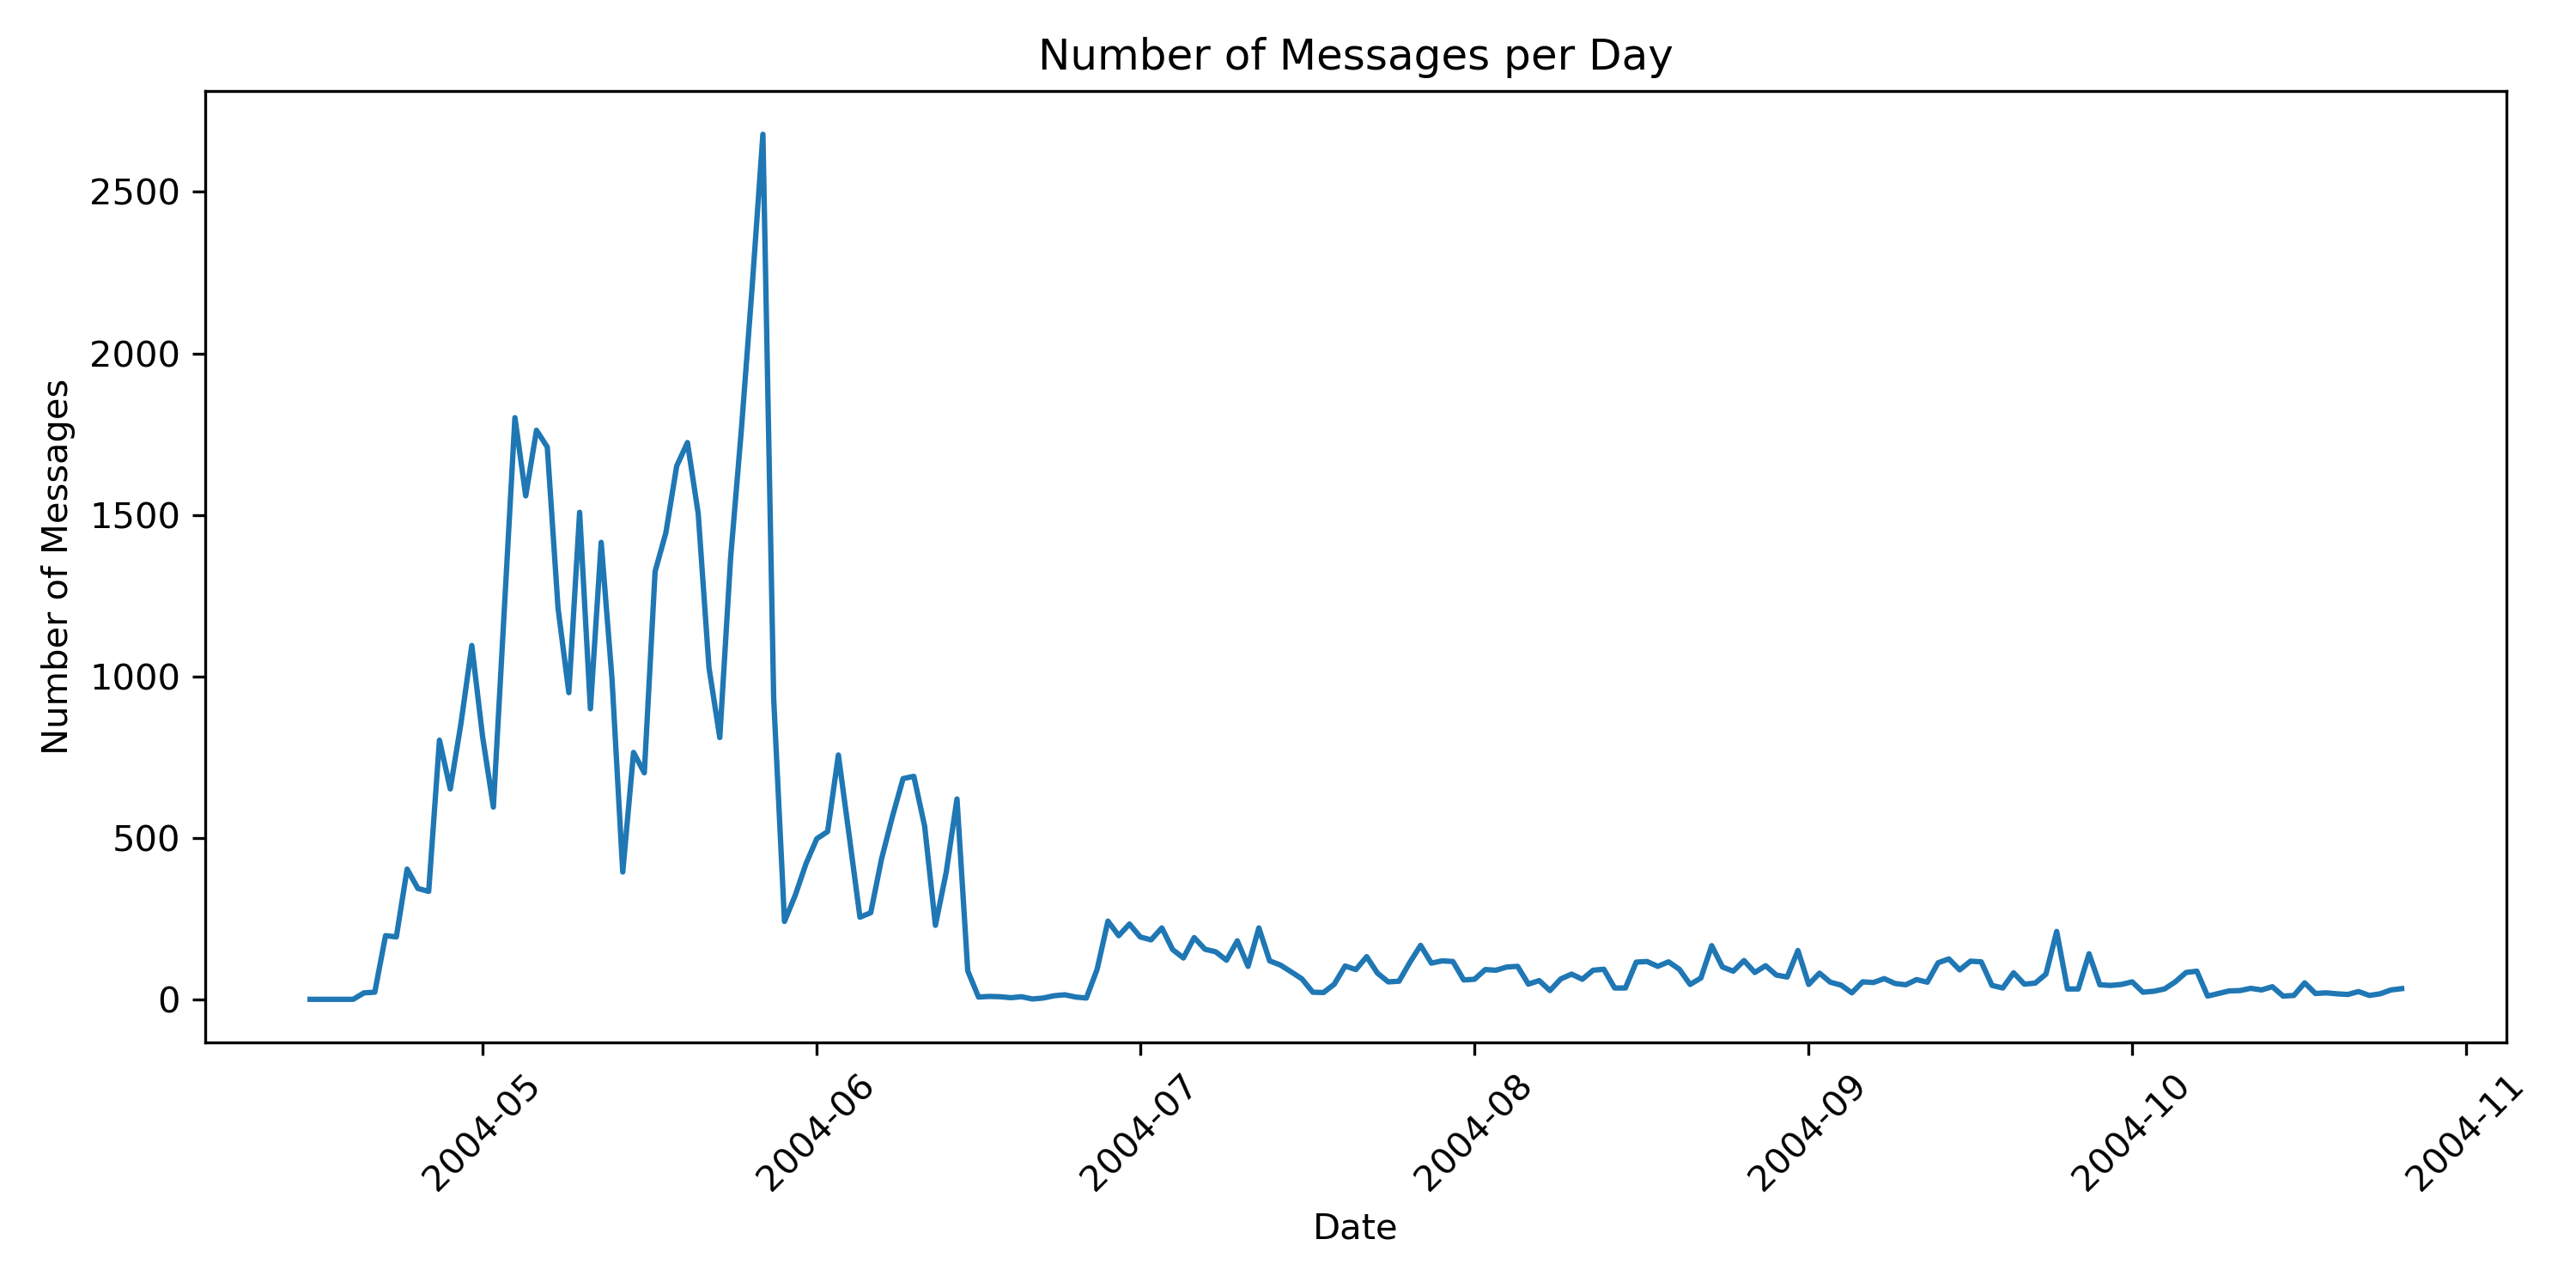
\includegraphics[width=0.5\linewidth]{../Images/messages_per_day.png}
    \caption{Daily message volume over time}
    \label{fig:messages-per-day}
\end{figure}

\subsection{Temporal Analysis}

During the preliminary analysis of hourly messaging patterns, an anomaly was noted: a substantial number of messages appeared to be sent between 5:00 and 8:00 a.m. UTC—an unusual timeframe for student activity.

This observation suggested a potential misalignment between recorded and actual local times. Considering the dataset originates from UC Irvine, the hypothesis emerged that timestamps required conversion to Pacific Time. Upon applying this correction, the messaging peak appropriately shifted to between 10:00 a.m. and 1:00 p.m.

To develop a comprehensive understanding of temporal behavior, message frequencies were further analyzed across hours of the day, weekdays, and months. The resulting trends are presented collectively in Figure~\ref{fig:temporal-analysis}.

\begin{figure}[H]
    \centering
    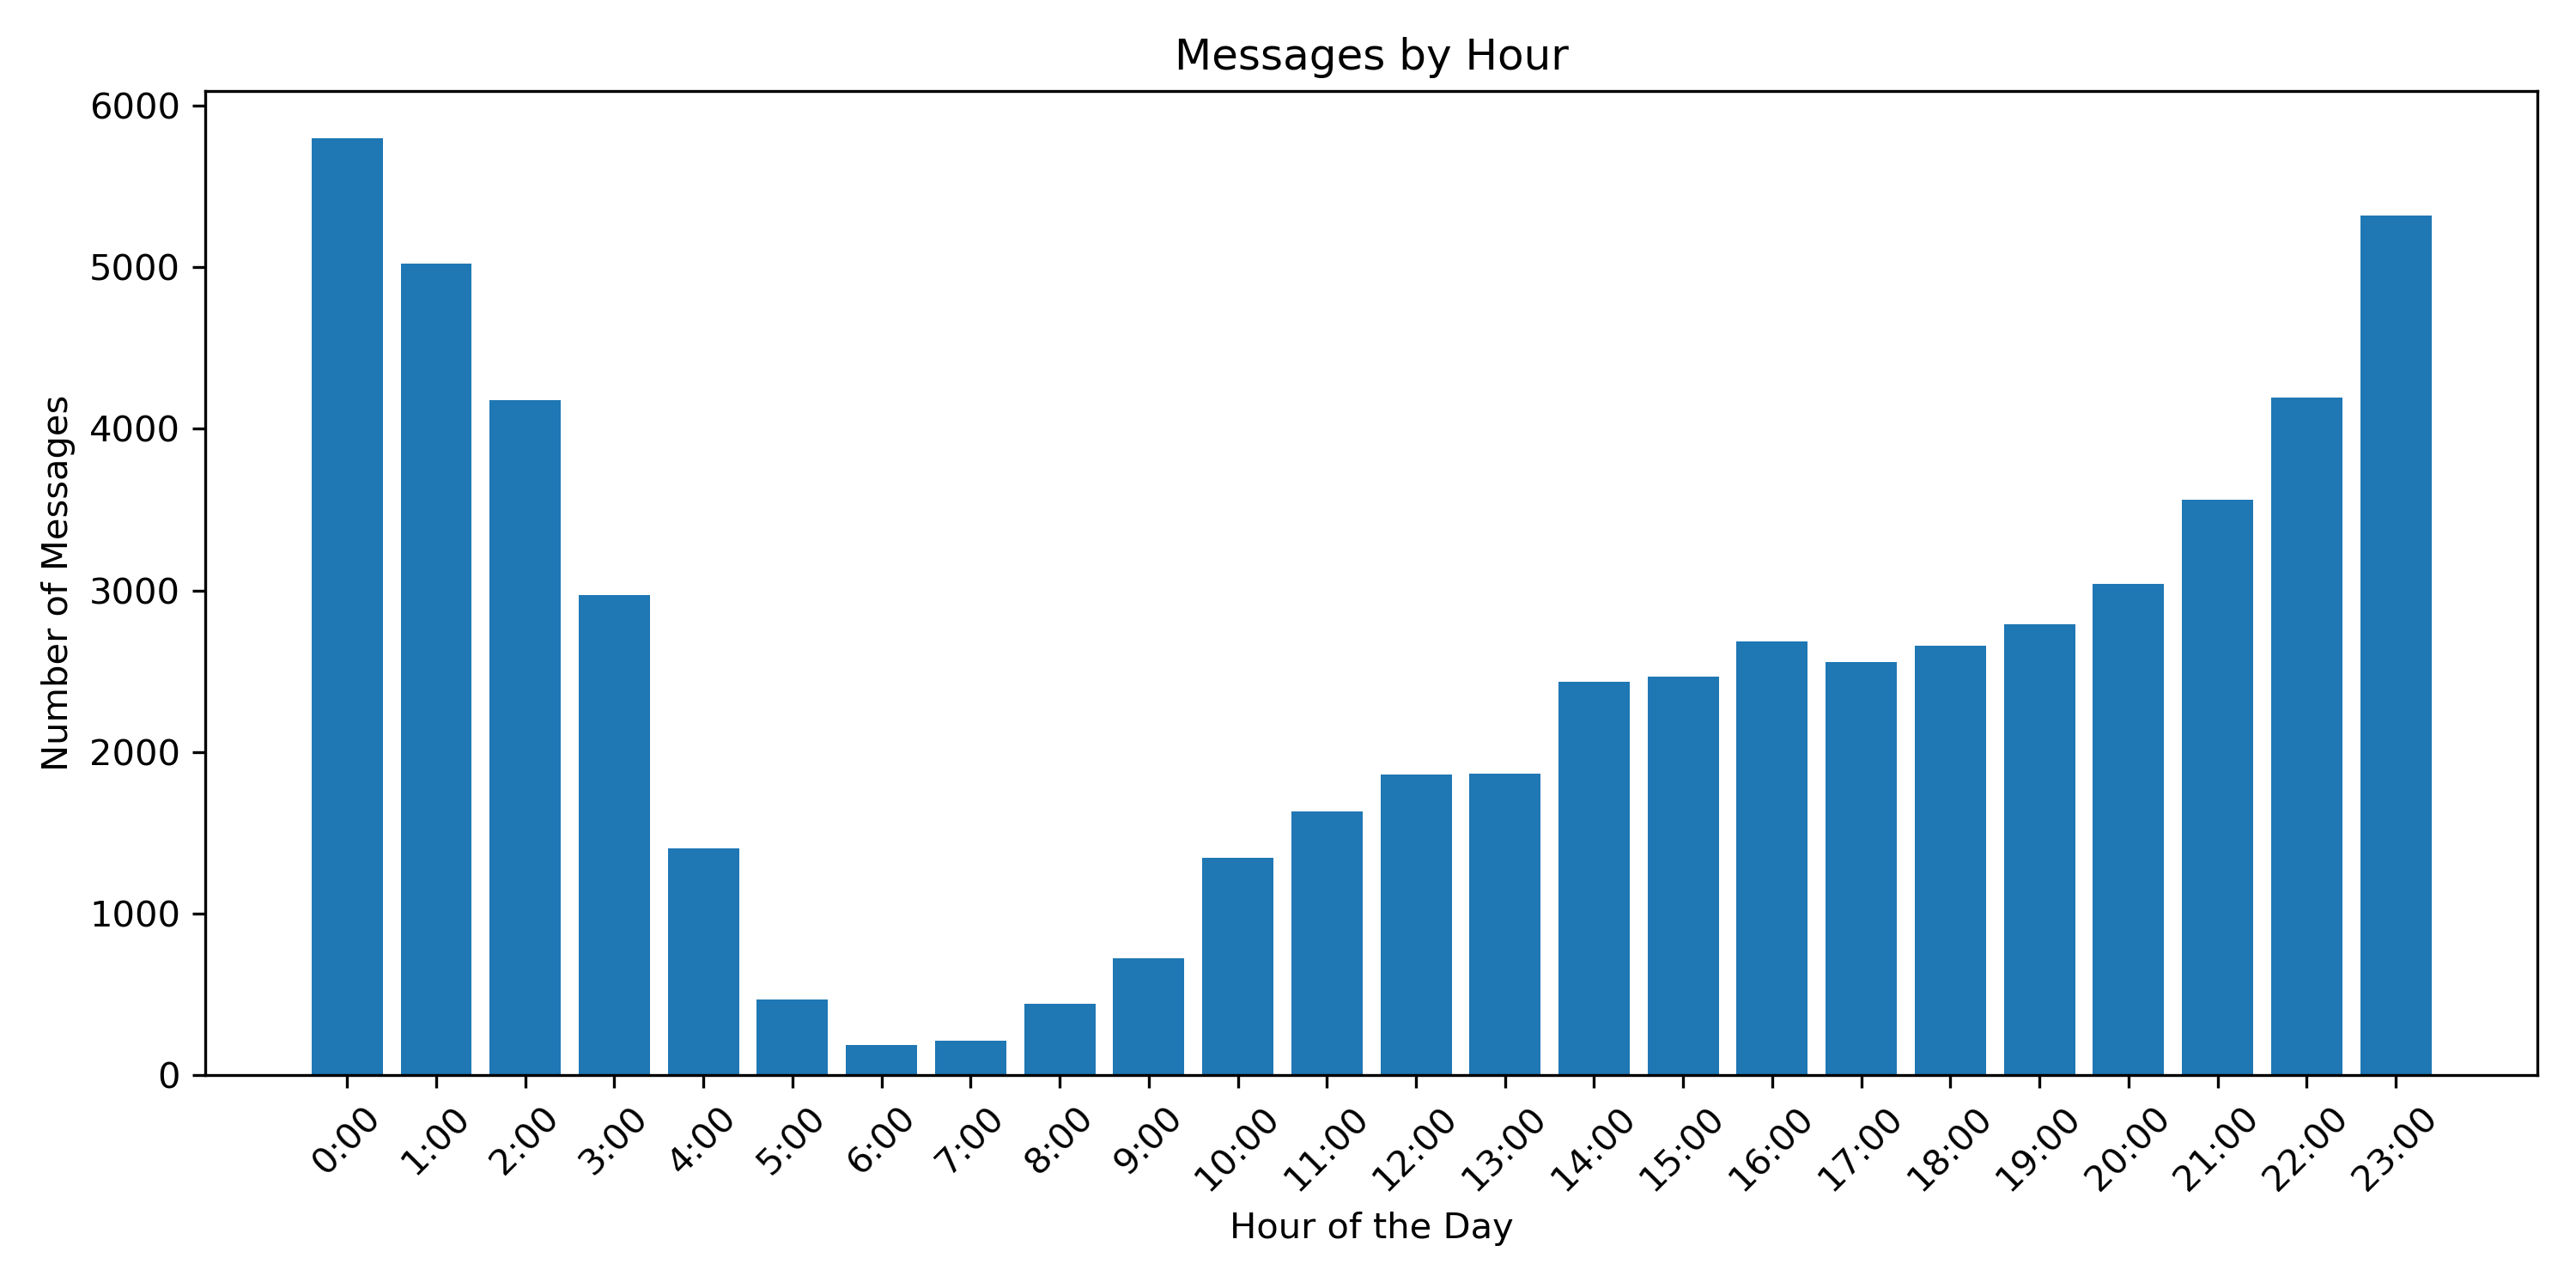
\includegraphics[width=0.3\linewidth]{../Images/messages_by_hour.png}
    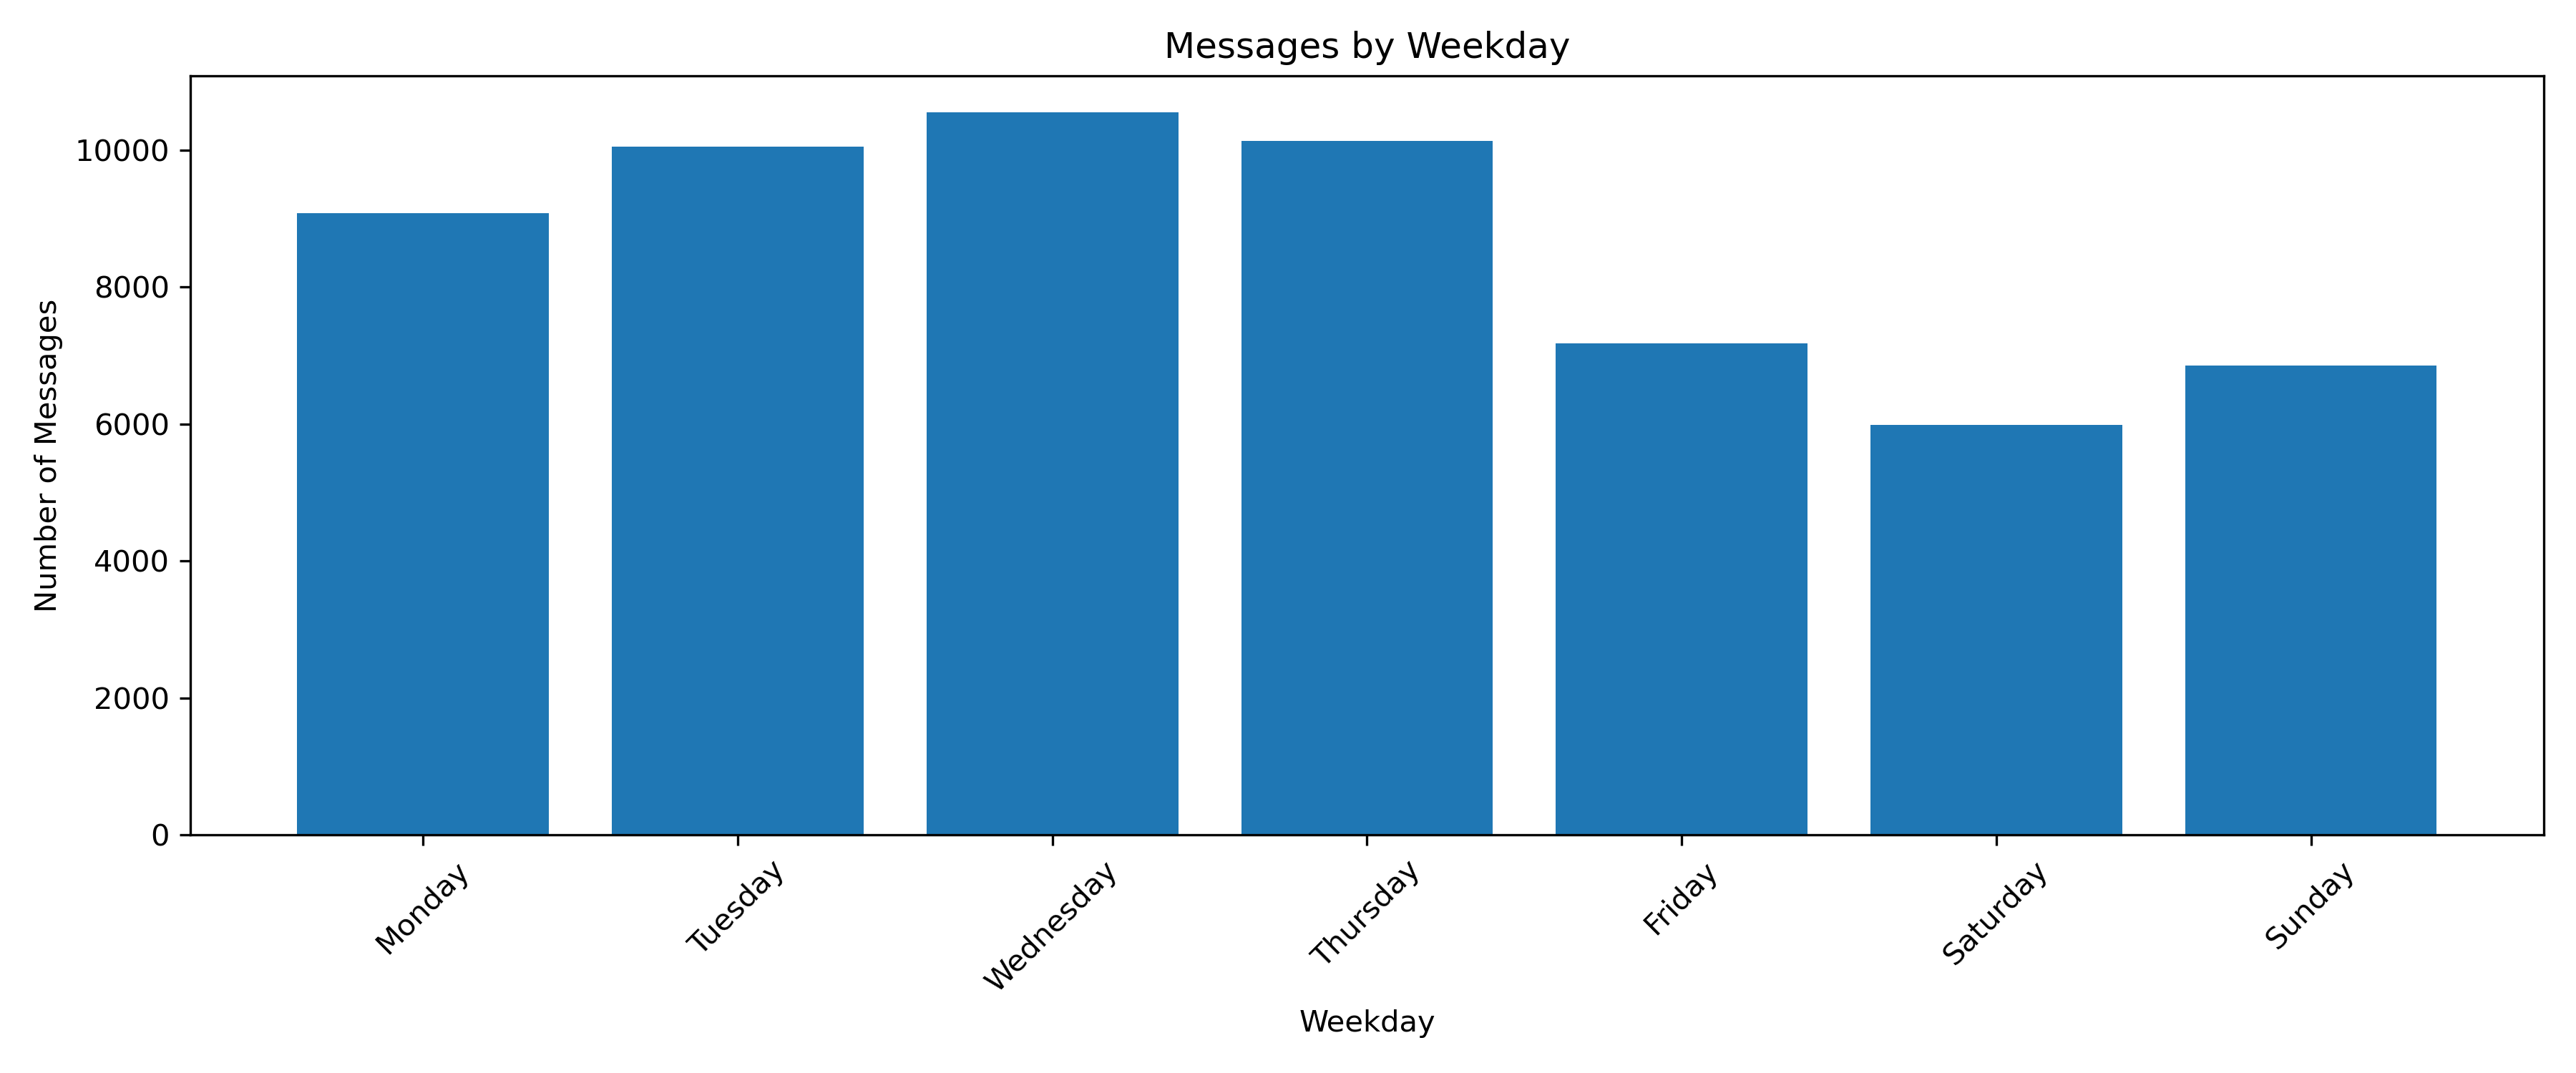
\includegraphics[width=0.3\linewidth]{../Images/messages_by_weekday.png}
    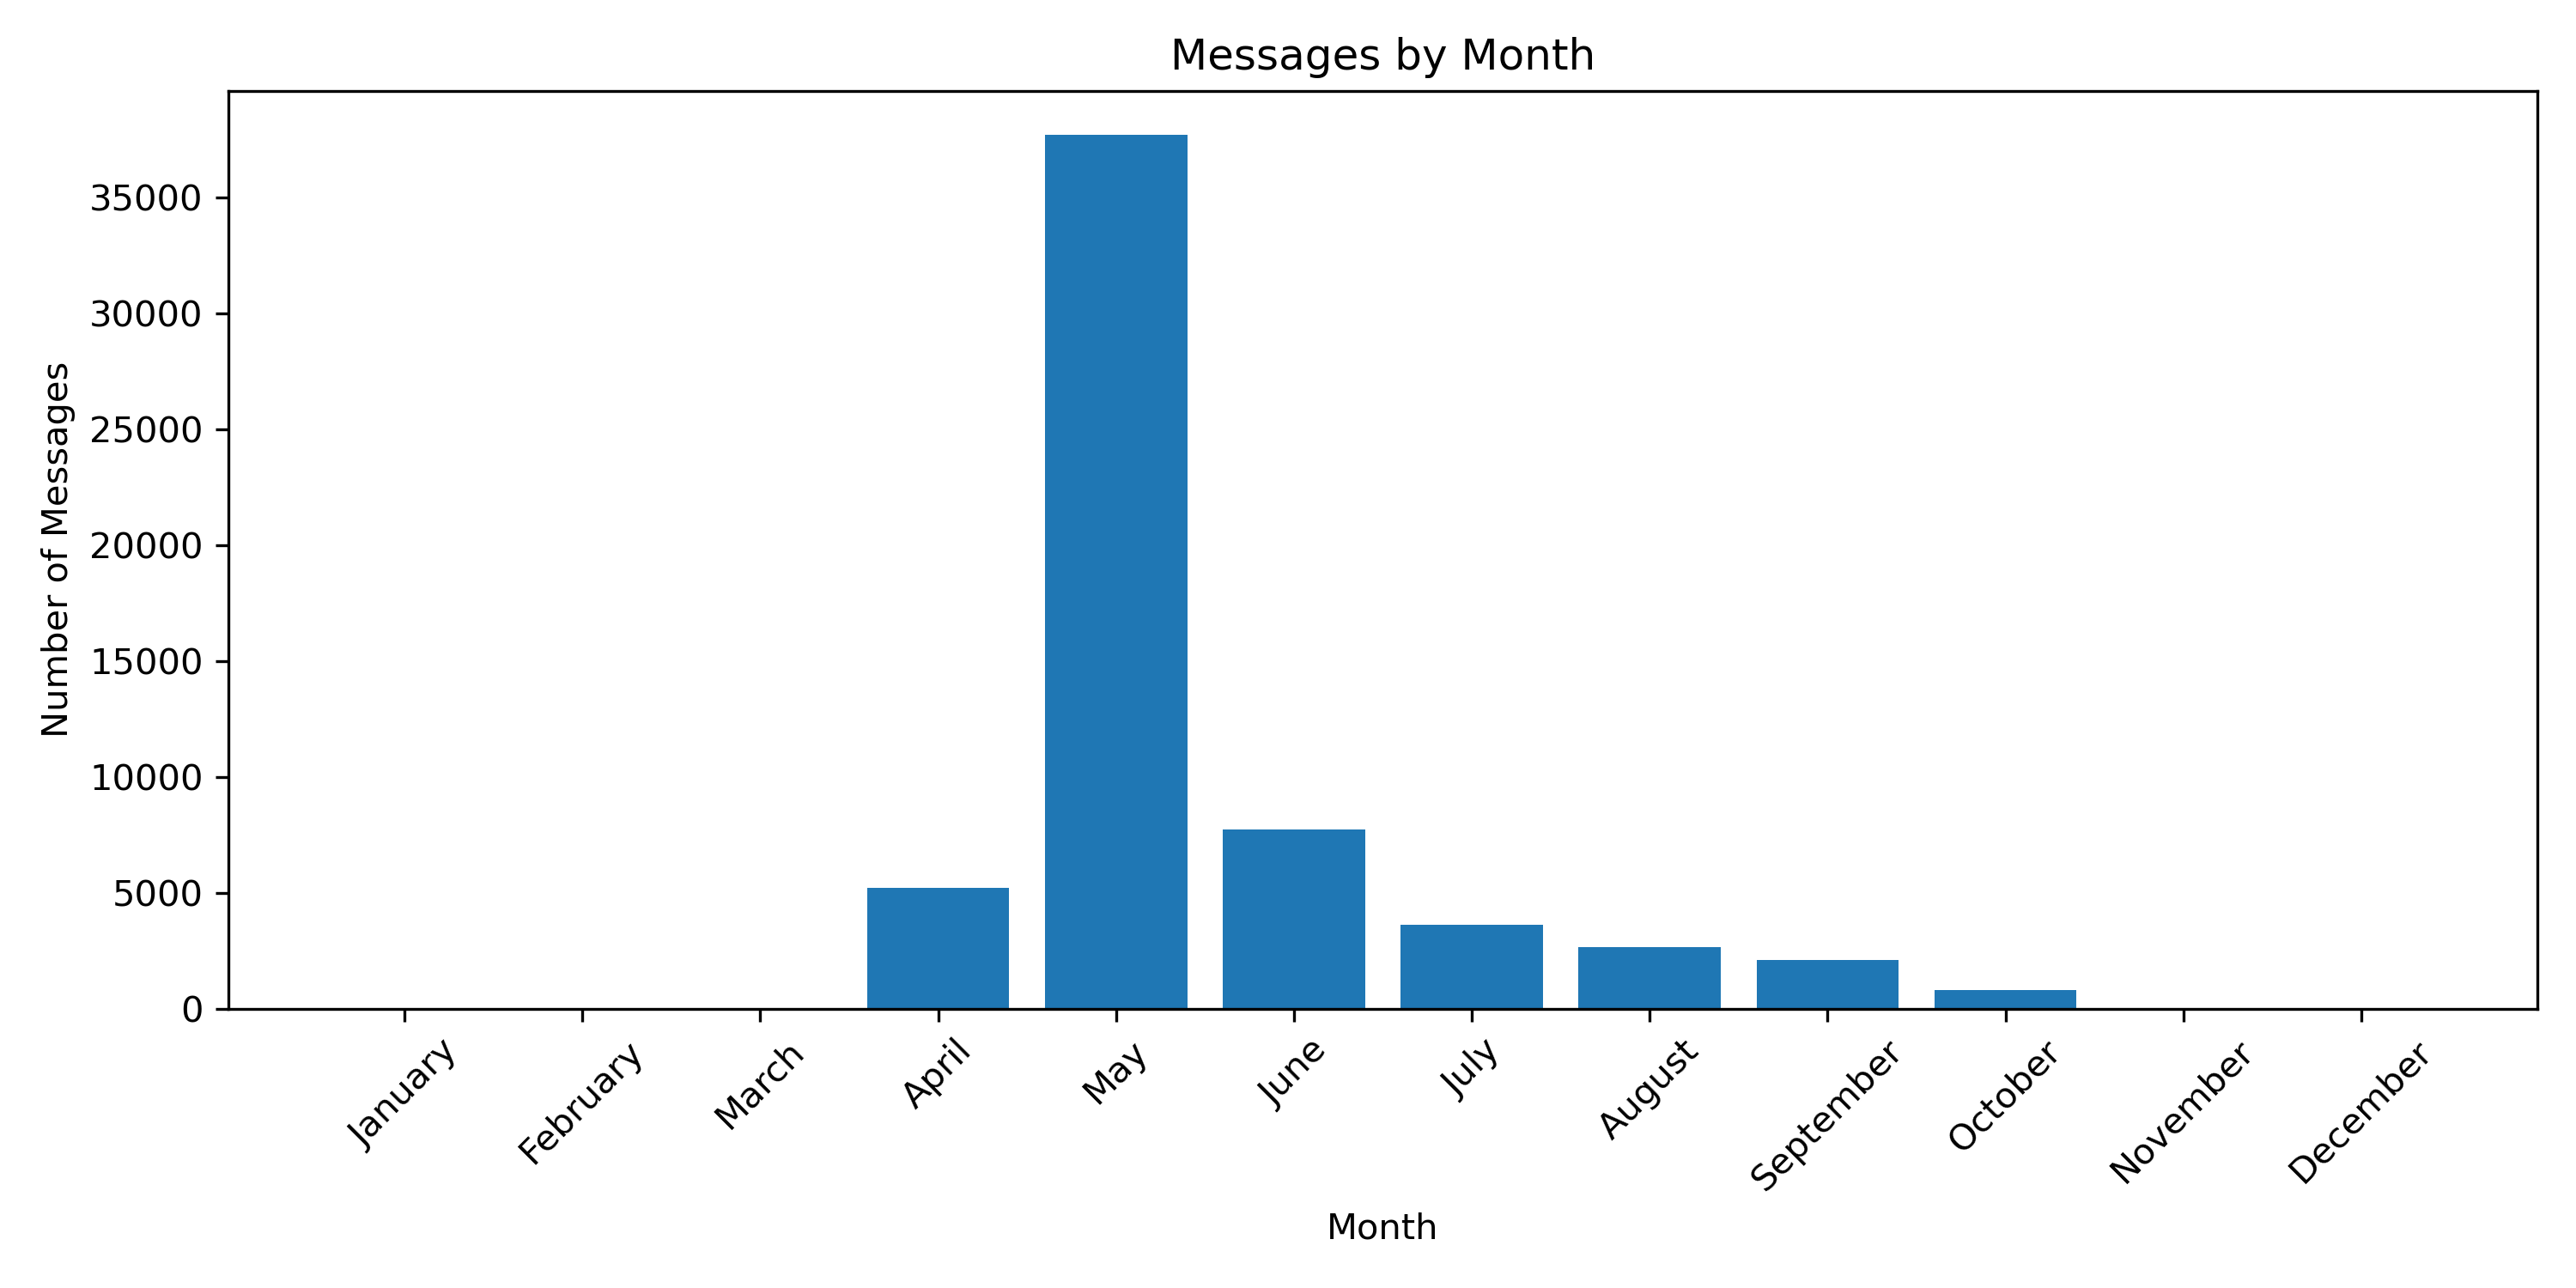
\includegraphics[width=0.3\linewidth]{../Images/messages_by_month.png}
    \caption{Temporal breakdown of message activity by hour, weekday, and month (adjusted to local time)}
    \label{fig:temporal-analysis}
\end{figure}

The analysis reveals heightened activity during mid-morning to early afternoon, reduced interaction over weekends, and seasonal variations, with communication peaking in spring and early autumn—likely aligned with the academic calendar.

\subsection{Top Users vs Least Users Analysis}

Following the identification of User 234 as one of the most active participants, a question arose:

\textit{"Do highly central users demonstrate distinct behavioral patterns compared to less active ones?"}

To investigate this, PageRank scores were computed to identify the most and least central users. Subsequently, their hourly messaging distributions were analyzed.

\begin{figure}[H]
    \centering
    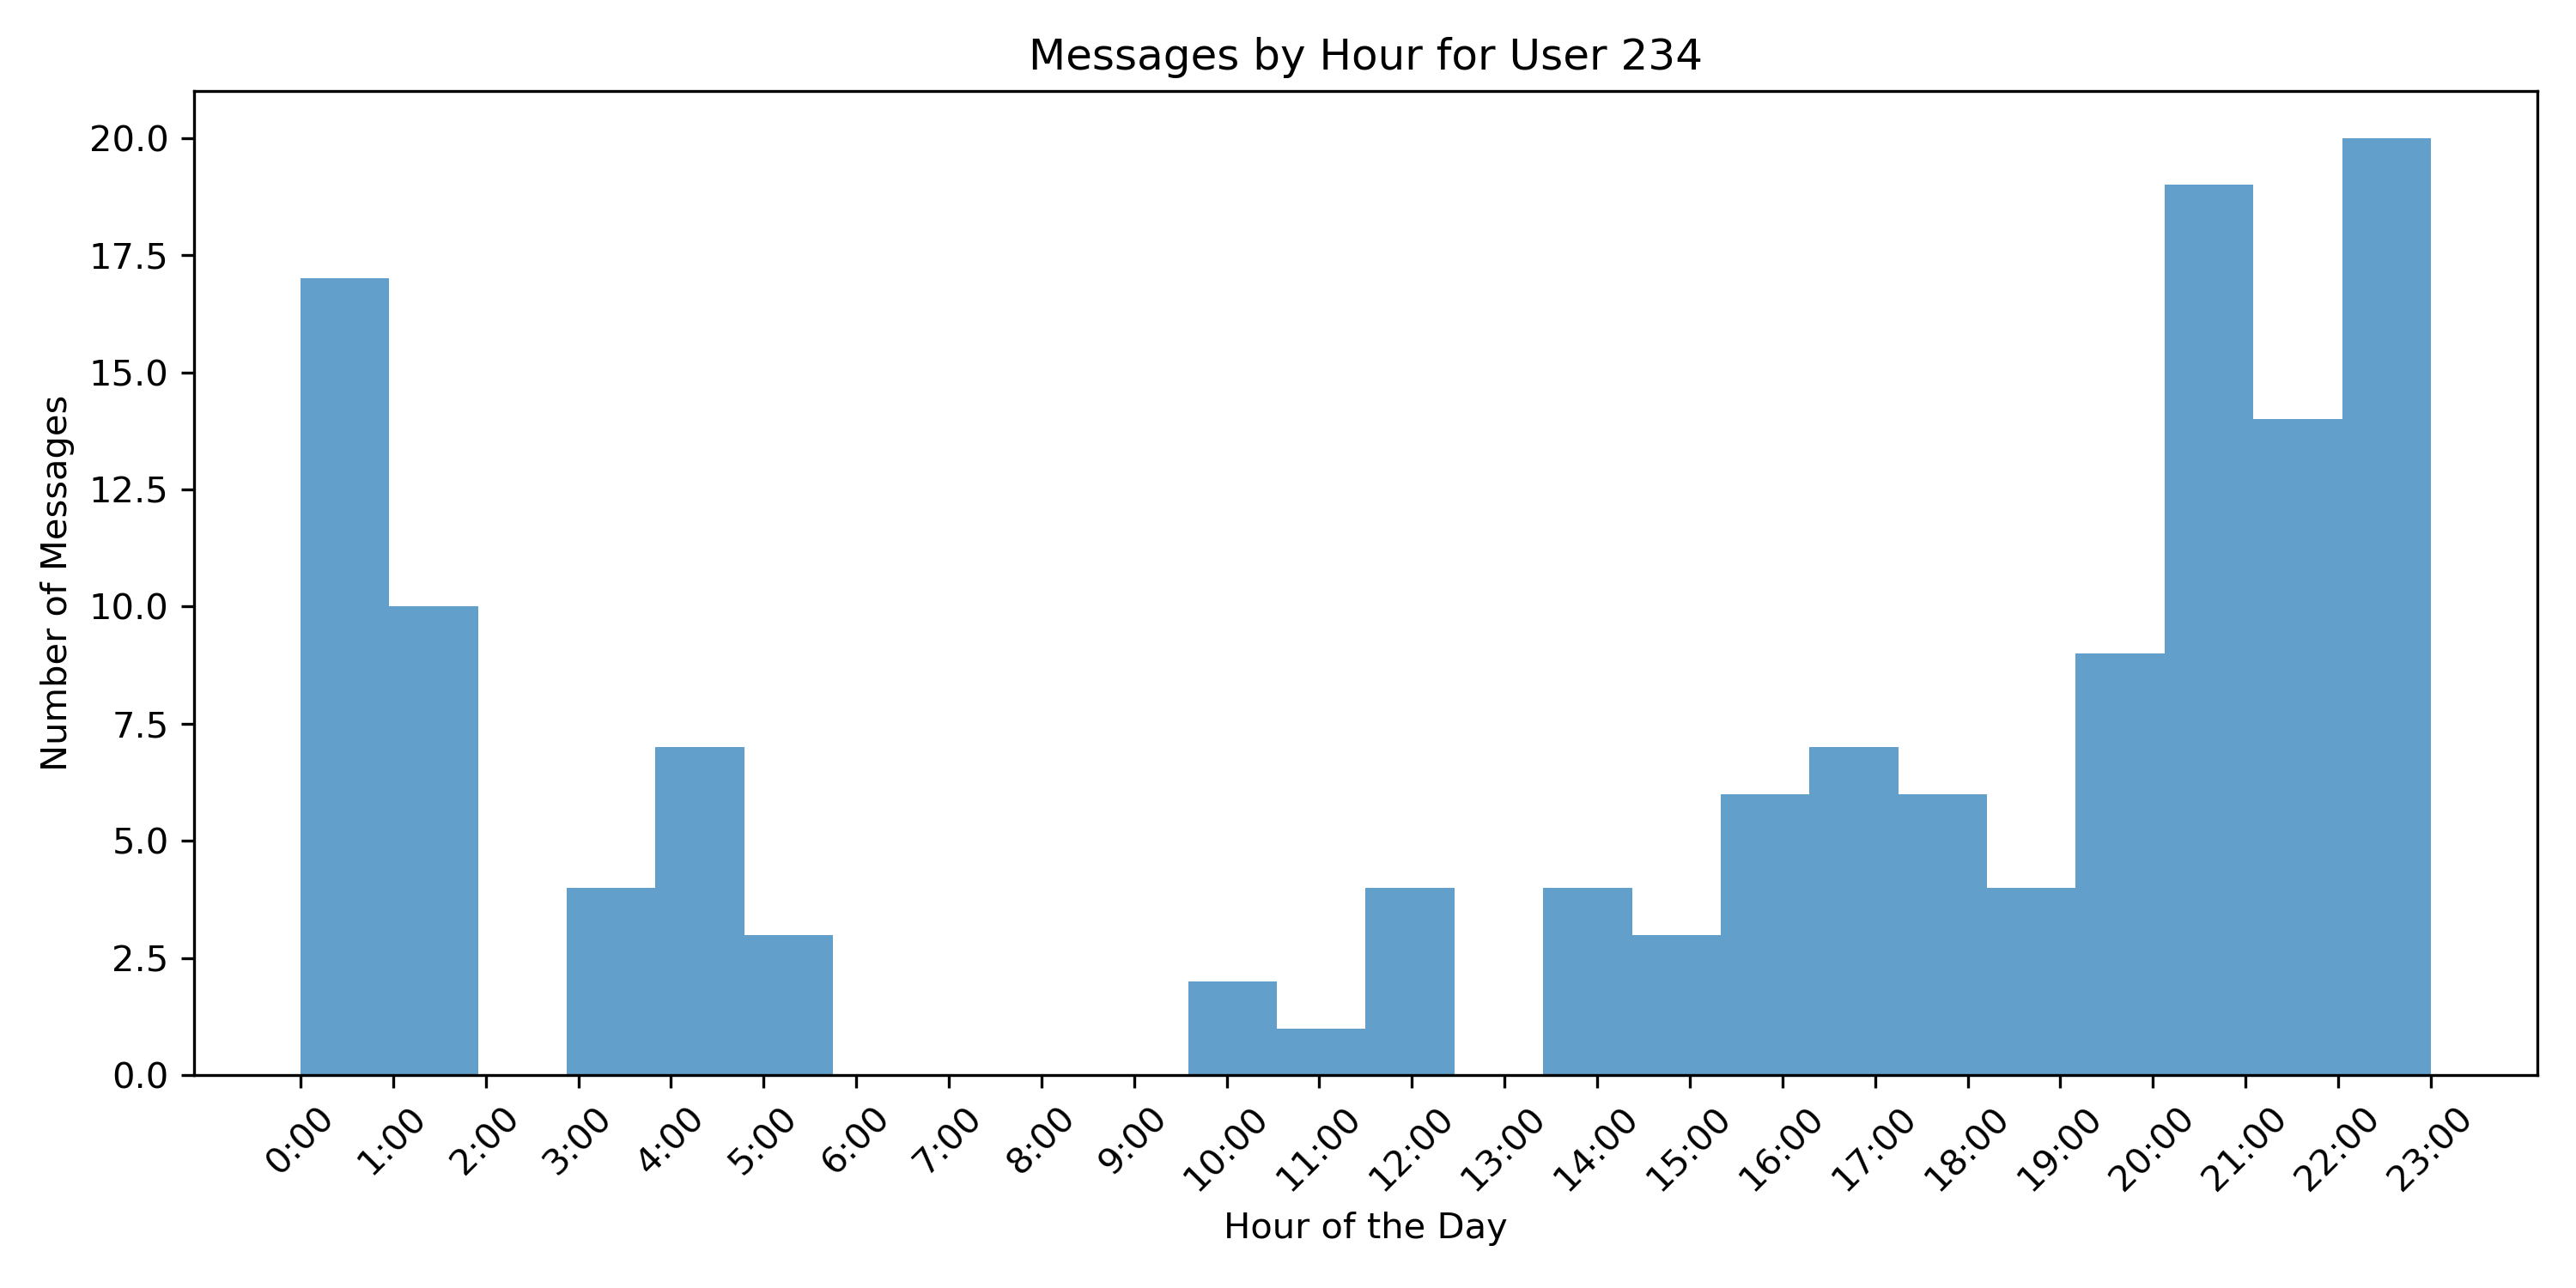
\includegraphics[width=0.6\linewidth]{../Images/user_234_messages_by_hour.png}
    \caption{Hourly message distribution for User 234}
    \label{fig:user234-hourly}
\end{figure}

As illustrated in Figure~\ref{fig:user234-hourly}, User 234 maintained a consistent level of activity throughout the day, with noticeable intensity in the evening—potentially indicating a central role within the network.

To broaden the perspective, the average hourly activity of the top 10 users (by PageRank) was compared against that of the bottom 1500 users.

\begin{figure}[H]
    \centering
    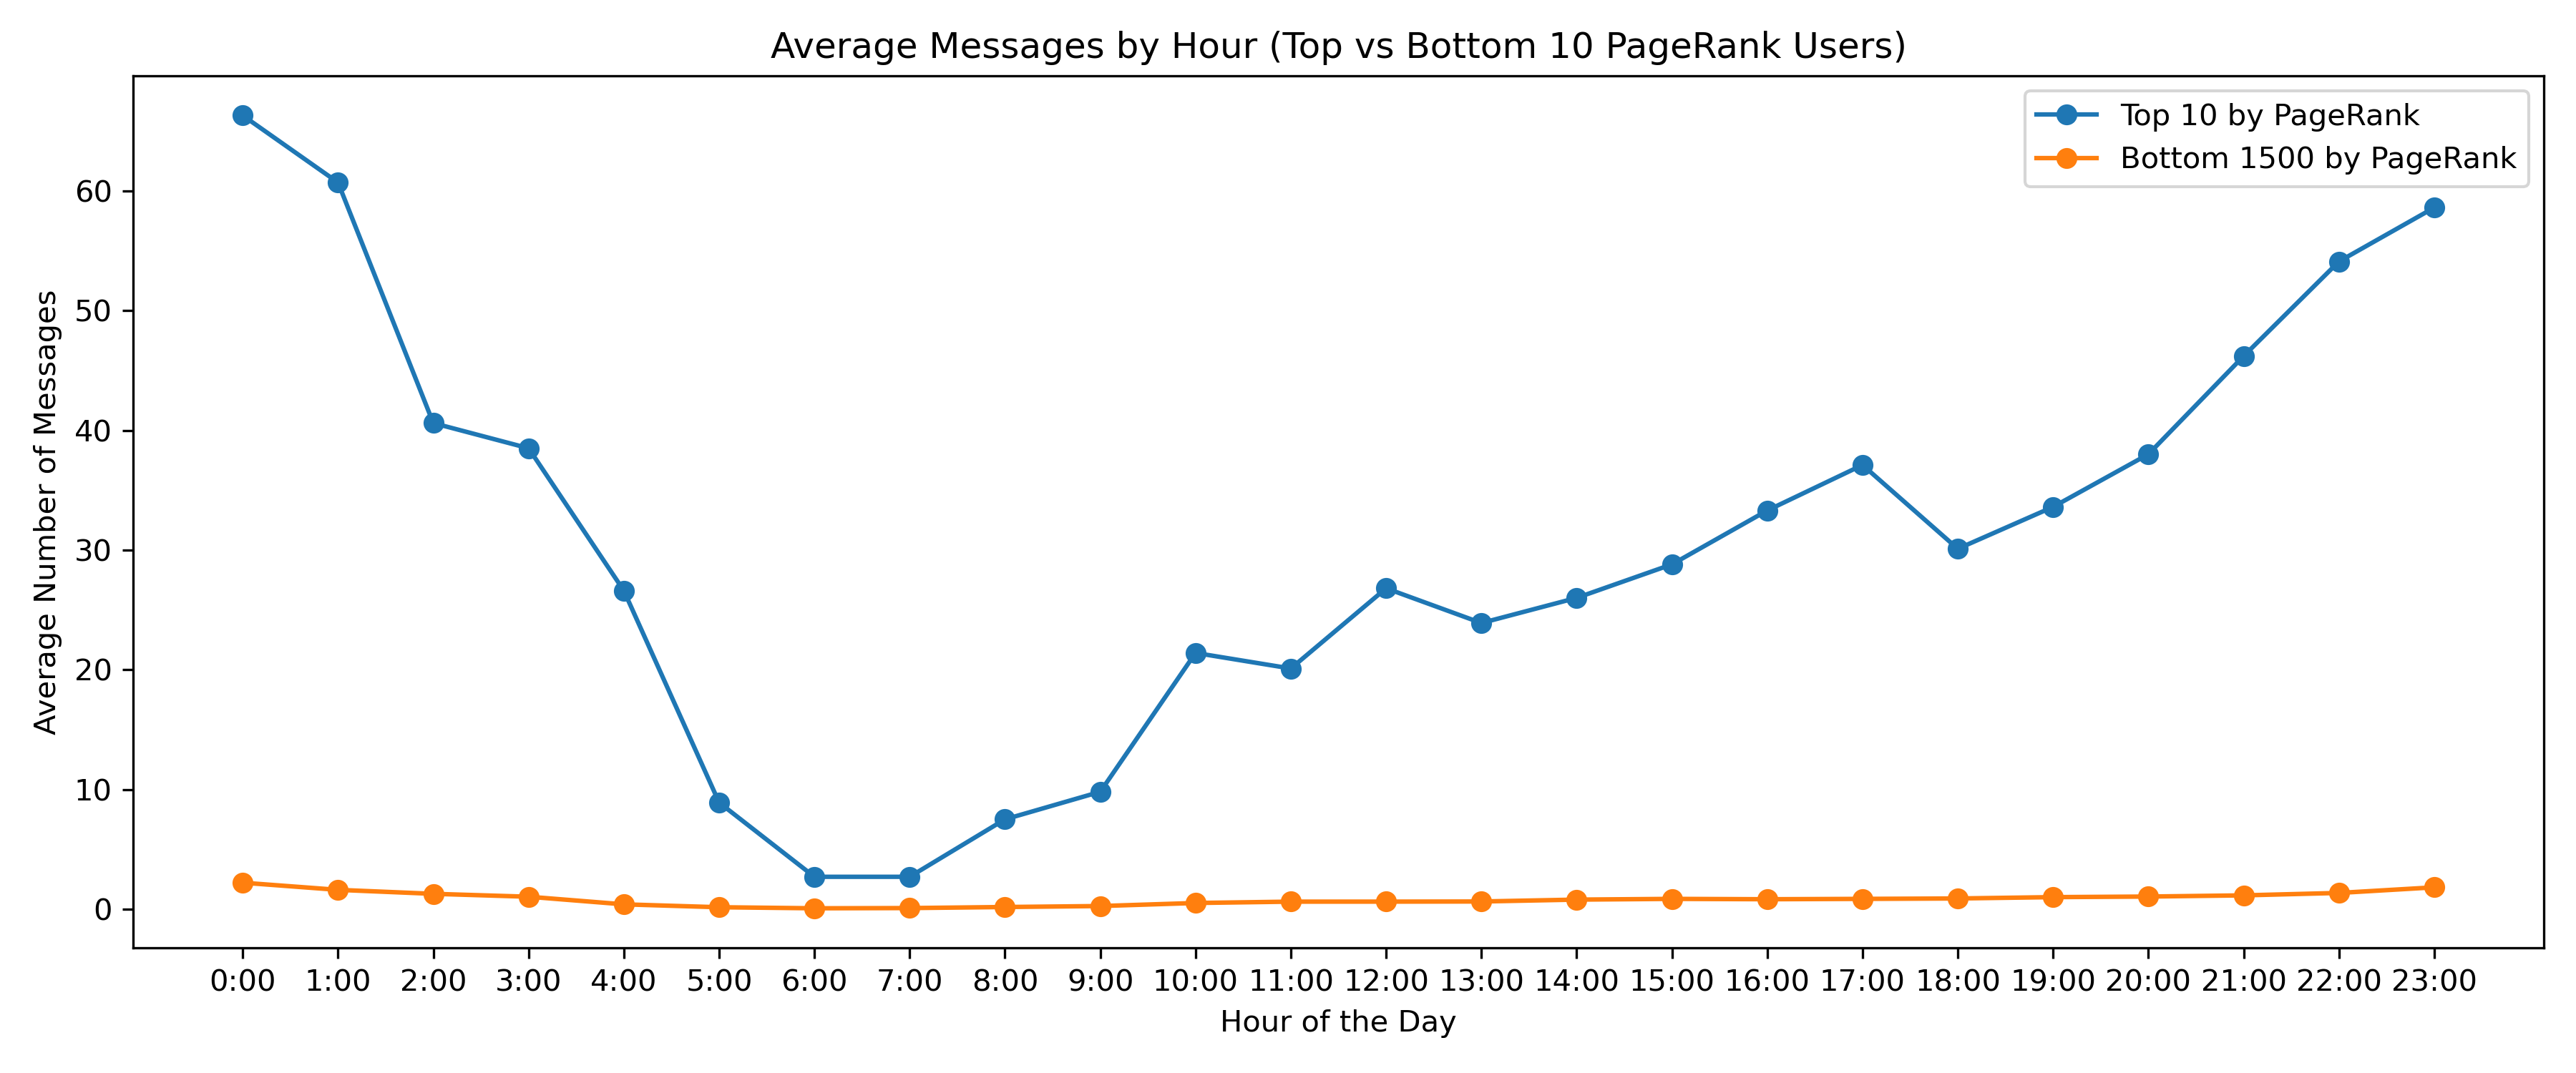
\includegraphics[width=0.5\linewidth]{../Images/average_messages_by_hour_top_bottom.png}
    \caption{Comparison of average hourly activity between top and bottom PageRank users}
    \label{fig:top-vs-bottom}
\end{figure}

As shown in Figure~\ref{fig:top-vs-bottom}, top-ranked users exhibited a more consistent and structured communication pattern, particularly active during typical daytime hours. In contrast, lower-ranked users displayed sporadic and irregular messaging behavior, further reinforcing the relevance of centrality in understanding user roles within the network.